\documentclass[14pt,a4paper]{extarticle}
\usepackage[utf8]{inputenc}
\usepackage[russian]{babel}
\usepackage{amsmath}
\usepackage{amsfonts}
\usepackage{amssymb}
\usepackage{setspace}
\usepackage[left=2.5cm, right=2cm, bottom=1.5cm, top=2cm]{geometry}
\usepackage{indentfirst}
\usepackage{tikz}
\usepackage{siunitx}
\usepackage{caption}
\usepackage{graphicx}
\usepackage{tabularx}

\usepackage{algpseudocode}
\usepackage{eqparbox}

\newcounter{algorithmic}
\newenvironment{myalgorithmic}[1][0]{\stepcounter{algorithmic}\begin{algorithmic}[#1]}{\end{algorithmic}}
\algrenewcommand{\algorithmiccomment}[1]{\hfill%
\eqparbox{COMMENT\thealgorithmic}{$\quad\rhd$\hspace{.5em}#1}%
}

\newcommand{\pd}[2]{\frac{\partial #1}{\partial #2}}
\newcommand{\dpd}[2]{\dfrac{\partial #1}{\partial #2}}

\newcommand{\pdd}[2]{\frac{\partial^2 #1}{\partial #2^2}}
\newcommand{\pddd}[3]{\frac{\partial^2 #1}{\partial #2\partial #3}}

\renewcommand{\arraystretch}{1.2}

\let\dividesymbol\div
\renewcommand{\div}{\operatorname{div}}
\newcommand{\grad}{\operatorname{grad}}
\newcommand{\rot}{\operatorname{rot}}
\newcommand{\const}{\operatorname{const}}
\newcommand{\diag}{\operatorname{diag}}
\renewcommand{\vec}[1]{\boldsymbol{\mathbf{#1}}}
\newcommand{\ten}[1]{\mathbf{#1}}
\newcommand{\cutefrac}[2]{{}^{#1}\mkern-5mu/{\!}_#2}
\newcommand{\half}{{\cutefrac{1}{2}}}
\renewcommand{\leq}{\leqslant}
\renewcommand{\geq}{\geqslant}

\newcommand{\n}[1]{\num[exponent-product=\cdot]{#1}}

\begin{document}

\thispagestyle{empty}

\newgeometry{left=1.5cm, right=1cm, bottom=1.5cm, top=2cm}

\begin{center}
	Министерство образования и науки Российской Федерации\\[6pt]
	
	Федеральное государственное автономное образовательное учреждение\\
	высшего профессионального образования\\
	<<Московский физико-технический институт (государственный университет)>>\\[6pt]
	
	Факультет управления и прикладной математики\\[6pt]
	Кафедра информатики и вычислительной математики\\[6pt]	
\end{center} 
\vspace{20mm}
\begin{flushright}
На правах рукописи\\
УДК 519.6
\end{flushright}

\begin{center}
	Гринин Виктор Олегович\\[6pt]
	
	{\large {\bf Моделирование многофазных реагирующих фильтрационных течений с равновесными химическими реакциями}}\\[6pt]
	
	Выпускная квалификационная работа\\
	(бакалаврская работа)\\
	
	Направление подготовки: 03.03.01 <<Прикладные математика и физика>>
\end{center}

\vspace{20mm}

\begin{flushleft}
	\begin{tabularx}{\textwidth}{lcl}
		Заведующий кафедрой: \\
		д.ф.-м.н., чл.-корр. РАН  & \raisebox{-3pt}{\rule{4cm}{0.5pt}} & Петров Игорь Борисович \\[5mm]
	
		Научный руководитель:\\
		к.ф.-м.н. & \raisebox{-3pt}{\rule{4cm}{0.5pt}} & Цыбулин Иван Владимирович \\[5mm]	
	
		Выполнил: \\
		Студент 373 группы  & \raisebox{-3pt}{\rule{4cm}{0.5pt}} & Гринин Виктор Олегович \\[5mm]
		
	\end{tabularx}
\end{flushleft}

\vfill

\begin{center}
	Москва, 2017
\end{center}

\onehalfspacing

\restoregeometry

\clearpage
\tableofcontents
\clearpage

\addcontentsline{toc}{section}{Введение}
\section*{Введение}

В настоящей работе рассматриваются многофазные фильтрационные течения, в которых наряду с реакциями с конечной кинетикой присутствуют равновесные химические реакции. Одним из приложений данных задач является изучение способов хранения углекислого газа в естественных подземных резервуарах. Для этого углекислый газ закачивают под давлением в водоносный горизонт, где газ будет находиться несколько сот лет. При этом газ может химически прореагировать с окружающей горной породой, что позволяет эффективно его связать. В данном случае химические превращения становятся важным аспектом такого фильтрационного течения.

Система химических реакций, описывающих взаимодействие углекислого газа с породой, обычно записывается в виде уравнений балансов отдельных ионов и веществ. Данные реакции имеют равновесный характер: их характерные времена  существенно меньше характерных времен фильтрации. Это обстоятельство осложняет учет реакций в разностной схеме, так как их нельзя учитывать последовательно с помощью метода расщепления: равновесие, достигнутое после учета только одной реакции будет нарушено при учете второй и так далее. Из-за этого все равновесные реакции требуется учитывать одновременно в единой системе уравнений.

При взаимодействии углекислого газа с породой, последняя растворяется, образуя дополнительный поровый объем. Это означает, что в модель фильтрационного течения должна быть заложена возможность учитывать изменяющуюся пористость резервуара. В имеющемся программном комплексе для моделирования многофазных многокомпонентных неизотермических течений, разработанном в лаборатории флюидодинамики и сейсмоакустики МФТИ, такая возможность имеется, так как в нем скелет рассматривается как отдельная фаза, участвующая в фазовых и химических превращениях. При таком подходе пористость является производным параметром, равным доле объёма, приходящейся на подвижные фазы.

Цель данной работы заключалась в усовершенствовании указанного программного комплекса в направлении учета
равновесных химических реакций, а также проведения численных экспериментов по закачке углекислого газа в модельный водный резервуар.

\clearpage
\section{Математическая модель}

Основными уравнениями, заложенными в программный комплекс \cite{shev}, которые описывают течение многофазной многокомпонентной среды являются уравнения балансов количества вещества и энергии, имеющие вид
\begin{gather*}
\pd{N_i}{t} + \div \vec Q_i = S_i,\\
\pd{E}{t} + \div \vec J = R.
\end{gather*}
Здесь $N_i$ --- молярные концентрации компонент, $E$ --- плотность энергии среды. Химические реакции учитываются в математической модели течения многофазной многокомпонентной среды в виде источников количества вещества $S_i$ и энергии $R$.

Молярные плотности и плотность энергии задаются соотношениями
\[
N_i = \sum_{\alpha} \theta_\alpha n_\alpha x_{i,\alpha},\qquad
E = \sum_{\alpha} \theta_\alpha n_\alpha e_{\alpha},
\]
где $\theta_\alpha$ --- объемная доля фазы $\alpha$, $n_\alpha$ --- концентрация фазы $\alpha$, $x_{i,\alpha}$ --- молярная концентрация компоненты $i$ в фазе $\alpha$, $e_\alpha$ --- молярная энергия фазы $\alpha$.

Потоки вещества $\vec Q_i$ и энергии $\vec J$ выражаются в виде
\[
\vec Q_i = \sum_\alpha n_\alpha x_{i,\alpha} \vec W_\alpha, \qquad
\vec J = \sum_\alpha n_\alpha h_{\alpha} \vec W_\alpha,
\]
где $h_\alpha$ --- энтальпия фазы $\alpha$, а $\vec W_\alpha$ --- скорость фильтрации фазы $\alpha$, задаваемая законом Дарси
\[
\vec W_\alpha = K \frac{\kappa_\alpha}{\mu_\alpha} (-\grad p + \rho_\alpha \vec g).
\]
В этом уравнении $K$ --- проницаемость скелета, $\kappa_\alpha$ --- относительная фазовая проницаемость, $\mu_\alpha$ --- вязкость фазы $\alpha$, $p$ --- давление, $\rho_\alpha$ --- плотность фазы $\alpha$, $\vec g$ --- ускорение свободного падения.

\subsection{Уравнения химических реакций}

Для реакций с конечной скоростью обычно используется закон Арениуса, когда скорость реакции пропорциональна концентрациям реагирующих веществ в степенях их стехеометрических коэффициентов.
В случае равновесной химической реакции вместо скорости реакции имеется равновесное соотношение
$$F(N_i) = 0,$$
выражающее собой равенство скоростей прямой и обратной химических реакций.

Если записать равновесную химическую реакцию в виде 
$$\sum{\nu_i X_i} \rightleftharpoons 0,$$
где $X_i$ --- реагирующие вещества, а $\nu_i$ --- их стехеометрические коэффициенты в реакции, то для такой реакции принимается верным закон действующих масс:
$$
K = \prod_i N_i^{\nu_i}.
$$
Здесь предполагается, что $\nu_i$ для продуктов реакции положительны, а для реагентов --- отрицательны. 

В качестве функции $F$ для данной реакции можно взять 
$$F = \ln{K} + \sum{\nu_i \ln{N_i}}.$$
Пусть в силу  некоторых причин, например из-за переноса продуктов реакции течением, данное равновесие оказалось нарушено. Тогда из-за данной реакции концентрации изменяются по закону $$\Delta N_i = \xi \nu_i,$$ где $\xi$ --- величина, характеризующая глубину реакции, одинаковая для всех участвующих компонент.

Задача определения нового равновесия заключается в поиске такого значения $\xi$, что $F(N_i) = 0$.

 При этом, можно сделать очевидное обобщение на случай нескольких реакций
\begin{gather*}
N_i = N_i^0 + \sum_{j=1}^{M} \xi_j\nu_{i,j}\\
F_j(N_i)=\ln(K_j) + \sum_{i=1}^{M} \nu_{i,j}\ln{N_i} = 0
\end{gather*}
 
\subsection{Конкретные химические реакции}

\newcommand{\OHm}{\text{OH}^-}
\newcommand{\Hp}{\text{H}^+}
\newcommand{\WAT}{\text{H}_2\text{O}}
\newcommand{\CARB}{\text{CO}_2}
\newcommand{\Catwop}{\text{Ca}^{2+}}
\newcommand{\Calcite}{\text{CaCO}_3}
\newcommand{\HCO}{\text{HCO}_3^{-}}
При проведении расчётов использовалась следующая система химических реакций
\begin{align*}
R1:&\quad \OHm + \Hp \rightleftharpoons \WAT,\\
R2:&\quad \HCO +\Hp \rightleftharpoons \WAT + \CARB,\\
R3:&\quad \Calcite + 2\Hp \rightleftharpoons \WAT + \CARB + \Catwop.
\end{align*}

Эта  система может быть записана в матрично-векторной форме $$V^T Y \rightleftharpoons 0,$$ где
$$V^T =  \begin{Vmatrix}
-1 &0 &0  &1 &0 &-1 &0\\
0 &-1 &0  &1 &1 &-1 &0\\
0  &0 &-1  &1 &1 &-2 &1
		\end{Vmatrix}, \quad
  Y = \begin{Vmatrix}
  \OHm\\
  \HCO\\
  \Calcite\\
  \WAT\\
  \CARB\\
  \Hp\\
  \Catwop
  \end{Vmatrix}$$\\
или в виде таблицы Мореля\\
$$\begin{array}{|c|cccc|c|}
\hline
		&\WAT	&\Hp	&\CARB	&\Catwop	&\lg {K}\\
\hline
\OHm		&1		&-1		&0		  &0		&-14\\
%\hline
\HCO	&1		&-1		&1		  &0		&-5.928\\
%\hline
\Calcite		&1		&-2		&1		  &1		&-8.094\\
\hline
\end{array}$$

Данные числовые значения констант химического равновесия взяты из работы \cite{vostrikov}.

\clearpage
\section{Численный метод и программный модуль}

В основе численного метода, используемого в вычислительном комплексе, лежит полностью неявная дискретизация уравнений балансов количества вещества и энергии. Из уравнений балансов составляется единое уравнение для определения давления --- уравнение пъезопроводности, решаемое на каждом шаге по времени методом Ньютона. После нахождения очередного приближения для давления производится пересчет концентраций компонент и энергии. В данном подходе химические реакции являются одним из источниковых слагаемых в правой части уравнений.

Для того, чтобы добавить химическую реакцию в программный комплекс, необходимо вычислить <<глубину реакции>> --- количество элементарных актов реакции, которое необходимо провести, чтобы из данного состояния попасть в равновесное. Фактически, равновесная реакция моделируется как реакция со скоростью $S = \frac{\xi}{\tau}$, где $\xi$ --- глубина реакции, а $\tau$ --- шаг по времени. Таким образом, выбираются такие скорости реакции, что на следующем шаге по времени концентрации веществ оказываются в равновесном состоянии.

Для решения системы, которая описывает установление химического равновесия, использовался метод Ньютона. Были рассмотрены различные способы записи данной системы и был выбран оптимальный.

\subsection{Метод Ньютона с ограничением шага}

Запишем приведённую раньше систему в матричной форме
\footnote{Здесь и далее $\ln \vec x, \exp \vec x$ понимаются как результат покомпонентного применения функции к вектору.}
$$\vec{F}(\vec \xi) = \ln{\vec{K}} + V^T \ln{(\vec{N}^0 + V\vec \xi)} = 0$$
Продифференцируем эту функцию по $\vec \xi$
$$\frac{\partial \vec{F}}{\partial{\vec{\xi}}} = V^T\diag^{-1}(\vec{N}^0 + V\vec{\xi})V$$

Метод Ньютона с ограничением шага \cite{kalit} имеет вид
$$\vec{\xi}^{k+1} = \vec{\xi}^{k} - \alpha^{(k)}[V^T\diag^{-1}(\vec{N}^0 + V\vec{\xi})V]^{-1}(\ln{\vec{K}} + V^T \ln{(\vec{N}^0 + V\vec{\xi})}) \quad (1)$$
Для обычного метода Ньютона параметр $\alpha$ следует брать равным единице, однако итерации с $\alpha^{(k)} = 1$ могут привести к попаданию в область нефизических значений. В этом случае можно делать лишь часть шага метода Ньютона, выбирая параметр $\alpha$ из промежутка $[0, 1]$.   

При применении для численных расчётов метода Ньютона, работающего с системой уравнений, записанной в данном виде, возникает несколько проблем. Нужно выбирать начальное приближение $\vec{\xi}^0$ так, чтобы выражение под логарифмом было положительным $\vec{N}^0 + V\vec{\xi} > 0$. Для этого приходится решать систему линейных неравенств. Кроме того, на каждой итерации следует задавать параметр $\alpha^{(k)} \in [0,1]$ так, чтобы неравенства этой системы не нарушались.  
\begin{figure}[!h]
\begin{myalgorithmic}[1]
\Function{ChooseAlpha}{$\vec N_0, V, \vec \xi,\Delta \vec \xi$}
\State $\beta = 0.5$ \Comment {Множитель, обеспечивающий строгое условие $N > 0$}
\State $\alpha = 1 / \beta$
\State $\vec N = \vec N_0 + V \vec \xi$ \Comment {Значение концентраций на текущей итерации}
\State $\Delta \vec N = V \Delta \vec \xi$ \Comment {Поправка к концентрациям}
\For {$i = \overline{1,n}$} 
\If {$N_i + \alpha \Delta N_i < 0$}\Comment {Возможно лишь при $\Delta N_i < 0$}
\State $\alpha = -\frac{N_i}{\Delta N_i}$ \Comment {Уменьшаем $\alpha$}
\EndIf
\EndFor
\State \Return $\beta \cdot \alpha$
\EndFunction
\end{myalgorithmic}
\caption{Алгоритм выбора множителя шага $\alpha$}
\end{figure}

Алгоритм выбора параметра $\alpha$ устроен таким образом, чтобы гарантировать выполнение условий:
\begin{itemize}
\item $\alpha \in (0, 1]$.
\item Для каждой компоненты $i$ выполняется условие $N_i + \alpha \Delta N_i > 0$, причем неравенство выполняется <<с запасом>>.
\item Если для каждой компоненты $i$ условие $N_i + \Delta N_i > 0$ выполнено с запасом, то значение $\alpha$ в точности равно 1, т.е. метод превращается в обычный метод Ньютона.
\end{itemize}

\subsection{Метод Ньютона для расширенной системы}

Перепишем систему в другом виде, для этого введём дополнительные переменные $$\vec{p} = \ln{(\vec{N}^0 + V\vec{\xi})}$$ 

При этом получаем расширенную систему
$$\begin{cases} 
	\vec{F} = \ln{\vec{K}} + V^T\vec{p}=0,\\
	\exp(\vec{p})=\vec{N}^0 + V\vec{\xi}.
	
\end{cases}$$

Перенося все слагаемые в левую часть, получаем
$$\begin{cases} 
	\ln{\vec{K}} + V^T\vec{p}=0,\\
	\vec{N}^0 + V\vec{\xi} - \exp(\vec{p}) = 0.
\end{cases}$$
Эта система полностью эквивалентна исходной. Её можно записать в виде
$\vec{\Phi}(\vec{x}) = 0$, где $ \vec{x} = [\vec{\xi}, \vec{p}]$

Тогда метод Ньютона принимает вид\\
$$\vec{x}^{k+1} = \vec{x}^{k} - \alpha^{(k)}\left(\pd{\vec{\Phi}}{\vec{x}}\right)^{-1}\vec{\Phi}(\vec x^k) \quad (2)$$
 где $$\pd{\vec{\Phi}}{\vec{x}} = \begin{Vmatrix}
 0 & V^T \\
 V & -\diag({\exp(\vec{p})})
\end{Vmatrix}  $$
Использование метода Ньютона, переписанного в такой форме, уже не встречает проблем, характерных предыдущей версии. Как показывает эксперимент, он сходится из любого начального приближения, при любых начальных концентрациях. Кроме того, в данном случае можно выбрать $\alpha^{(k)} = 1$, что обеспечивает большую скорость сходимости.

Модуль, реализующий метод Ньютона в такой форме, был включён в симулятор многофазных фильтрационных течений. 

\clearpage
\section{Результаты}
\subsection{Верификация написанного модуля}
Приведём результаты расчётов системы из трёх химических реакций 
\begin{align*}
R1:&\quad \OHm + \Hp \rightleftharpoons \WAT,\\
R2:&\quad \HCO +\Hp \rightleftharpoons \WAT + \CARB,\\
R3:&\quad \Calcite + 2\Hp \rightleftharpoons \WAT + \CARB + \Catwop.
\end{align*}

Будем считать, что начальные концентрации всех ионов равнялись нулю, и вектор концентраций химических веществ имел вид
$$\vec{N}_0^T = [0, 0, 1, 1, 1, 0, 0]$$

В методе Ньютона, записанном для равновесной системы в форме $(1)$, начальное приближение искомых глубин реакции выбираем так, чтобы выполнялось условие $$\vec{N}^0 + V\vec{\xi} > 0.$$ Пусть например, $$\vec{\xi}_0^T = [-0.5, -0.7, 0.5]$$ 
\begin{table}[ht!]
	\caption{Концентрации веществ и выбираемый параметр $\alpha$ на соответствующей итерации метода Ньютона, записанного в форме $(1)$.}
	\small
	\begin{center}
	\begin{tabular}{|p{0.33cm}|p{1.7cm}|p{1.7cm}|p{1.7cm}|p{1.7cm}|p{1.7cm}|p{1.7cm}|p{1.7cm}|l|}
	\hline
		&$\OHm$	&$\HCO$ &$\Calcite$ &$\WAT$ &$\CARB$ &$\Hp$ &$\Catwop$ &$\alpha$\\
\hline
	1	&0	&0	&1  &1	&1	&0	&0	&0.05\\
%\hline
	2	&0.5	&0.7	&0.5 &0.3	&0.8 &0.06	&0.2	&0.06	\\
%\hline
	4	&0.12   &0.75  &0.60  &0.51 &0.63  &0.09 &0.39	&0.06\\
%\hline
	8	&\n{7.8e-03}   &\n{6.4e-01}  &\n{6.9e-01}  &\n{6.6e-01}  &\n{6.6e-01}  &\n{3.4e-02} &\n{3.1e-01}	&0.09\\
%\hline
	16	&\n{1.5e-05}   &\n{3.6e-01}   &\n{8.2e-01}   &\n{8.2e-01} &\n{8.2e-01}   &\n{3.3e-03}   &\n{1.8e-01}	&0.88\\
%\hline
	30	&\n{ 5.9e-10}    &\n{6.7e-02 }    &\n{9.7e-01 }    &\n{9.7e-01   } &\n{9.7e-01} &\n{1.6e-05  }  &\n{3.4e-02}	&1\\
\hline
	
\end{tabular}
\end{center}
\end{table}

Видим, что в результате химических реакций концентрации исходных веществ немного уменьшаются, в результате чего образуются все входящие в реакции ионы. 

На начальных итерациях выбирается $\alpha < 1$. Это говорит о том, что метод Ньютона пытается выйти за допустимую область. В результате ограничения шага в этом случае сходимость является линейной, и метод Ньютона работает как метод простой итерации. 

Для расширенной системы, как уже говорилось, $\alpha$ выбирается равным единице. Начальные значения $\xi_i$ можно выбрать произвольными. Пусть они будут такими же как в предыдущем случае.
\begin{table}[ht!]
	\caption{Концентрации веществ на соответствующей итерации метода Ньютона, записанного в форме $(2)$.}
	\small
	\begin{center}
	\begin{tabular}{|p{0.33cm}|p{1.7cm}|p{1.7cm}|p{1.7cm}|p{1.7cm}|p{1.7cm}|p{1.7cm}|p{1.7cm}|l|}
	\hline
		&$\OHm$	&$\HCO$ &$\Calcite$ &$\WAT$ &$\CARB$ &$\Hp$ &$\Catwop$ \\
\hline
	1	&0	&0	&1  &1	&1	&0	&0	\\
%\hline
	2	&\n{0.7}	&\n{1.9}	&\n{0.3}	&\n{0.8}	&\n{0.5}	&\n{1.0}	&\n{1.0}	\\
%\hline
	4	&\n{6.0e-09}      &\n{1.7}      &\n{3.6}      &\n{4234.8}    &\n{2.3} &\n{7e-03}      &\n{2.2}\\
%\hline
	8	&\n{2.6e-09}    &\n{2.6e-01}   &\n{8.7e-01}      &\n{78.1}    &\n{8.7e-01} &\n{3.1e-04 }     &\n{1.5e-01}\\
%\hline
	12	 &\n{7.6e-10}    &\n{8.6e-02 }    &\n{9.6e-01 }     &\n{ 2.1  }   &\n{9.6e-01} &\n{2.7e-05}    &\n{4.3e-02}\\
%\hline
	16	&\n{ 5.9e-10}    &\n{6.7e-02 }    &\n{9.7e-01 }    &\n{9.7e-01   } &\n{9.7e-01} &\n{1.6e-05  }  &\n{3.4e-02}\\
\hline
	
\end{tabular}
\end{center}
\end{table}

И для исходной системы, и для расширенной метод Ньютона сходится к одному и тому же значению. При этом, в случае расширенной системы требуется меньшее количество итераций.
\subsection{Применение модуля в симуляторе}
Разработанный алгоритм был включён в симулятор и использован для моделирования многофазных фильтрационных течений с химическими реакциями.

Одним из расчётных сценариев стала следующая задача. В ней рассматривается вытеснение углекислым газом воды из пористой области, скелет которой составляет углекислый кальций. 

Геометрия задачи такова
$$
\tikz {
\draw (0,0) --  +(10,0) -- +(10,2) -- +(0, 2) -- +(0,0);
\filldraw[fill=blue!20!white, draw=blue] (1,0) --  (16,0) -- (16,2) -- (1, 2) -- (1,0);
\filldraw[fill=blue!5!white, draw=blue] (0,0) --  (1,0) -- (1,2) -- (0, 2) -- (0,0);
\draw[dashed, gray] (0,0.25) -- (16,0.25); 
\draw[dashed, gray] (0,0.5) -- (16,0.5); 
\draw[dashed, gray] (1,0.75) -- (15,0.75); 
\draw[dashed, gray] (1, 1) -- (15, 1);
\draw[dashed, gray] (1,1.25) -- (15,1.25); 
\draw[dashed, gray] (0,1.5) -- (16,1.5); 
\draw[dashed, gray] (0,1.75) -- (16,1.75);
\draw[dashed, gray] (1,0) -- (1,2); 
\draw[dashed, gray] (2,0) -- (2,2); 
\draw[dashed, gray] (3,0) -- (3,2); 
\draw[dashed, gray] (4,0) -- (4,2); 
\draw[dashed, gray] (5,0) -- (5,2); 
\draw[dashed, gray] (6,0) -- (6,2); 
\draw[dashed, gray] (7,0) -- (7,2); 
\draw[dashed, gray] (8,0) -- (8,2);
\draw[dashed, gray] (9,0) -- (9,2);
\draw[dashed, gray] (10,0) -- (10,2); 
\draw[dashed, gray] (11,0) -- (11,2); 
\draw[dashed, gray] (12,0) -- (12,2); 
\draw[dashed, gray] (13,0) -- (13,2); 
\draw[dashed, gray] (14,0) -- (14,2); 
\draw[dashed, gray] (15,0) -- (15,2);
\draw [<->, orange] (0, -0.9) -- (16, -0.9); 
\draw [->, blue!20!white] (0, 2.2) -- (1, 2.2);
\fill
(0.5,1) node {inj}
(15.5,1) node {prod} 
(8,-0.6) node {L}
(0.5, 2.5) node {$\CARB$}
}
$$
Имеется область длины $L = 500 \text{ м}$. Поперечное сечение области $S = 10\times100 \text{ м}^2$. Пунктирной линией схематично показаны поры скелета, занятые водой. На концах области находятся скважины: cлева --- нагнетающая $(inj)$, справа --- добывающая $(prod)$. 

В области присутствуют две подвижные фазы: газовая и водная.
Предполагается следующее распределение компонентов по фазам:

Водная фаза: $ \WAT$, $ \CARB$, $ \OHm$, $ \HCO$, $ \Hp$, $ \Catwop$,

Газовая фаза: $\CARB $.

Кроме того, существует только одна неподвижная фаза, описывающая скелет и состоящая из углекислого кальция $\Calcite$.

При таком подходе пористость является производным параметром — отношением объема подвижных фаз к суммарному объему всех фаз.
Для рассматриваемой задачи задаётся начальная пористость $\phi = 0.05$.

Вязкости фаз считаются постоянными. 

Вязкость воды --- ${\mu}_W = 4.5 \cdot 10^{-3} \text{ Па} \cdot \text{с}$, газа --- $\mu_G = 2.09\cdot 10^{-5} \text{ Па} \cdot \text{с}$.

Относительные фазовые проницаемости задаются простым степенным законом $$k_{\alpha} = s_{\alpha}^2,$$ где $s_{\alpha}$ --- насыщенность подвижной фазы.

Начальная температура в области равна $20^\circ C$, начальное давление --- $100$ атмосфер. Хотя моделирование проводилось в неизотермическом режиме, температура в области остаётся практически постоянной, т.е. течение можно считать изотермическим.

Нагнетающая скважина закачивает в область углекислый газ с постоянным расходом $10^4 \text{ м}^3/\text{сут}$ (на поверхности, при 1 атмосфере), который постепенно вытесняет из области воду и частично растворяется в ней. Перенос жидкости и газа сопровождается химическими реакциями, описанными в предыдущих пунктах, в результате чего скелет растворяется, образуя ионы, которые вымываются из области. На рисунке \ref{fig:pic1} представлен график пористости в области в момент времени $t = 70\text{ дней}$. Видно, что часть скелета растворилась, образовав дополнительный поровый объем.

\begin{figure}[h!]
\centering
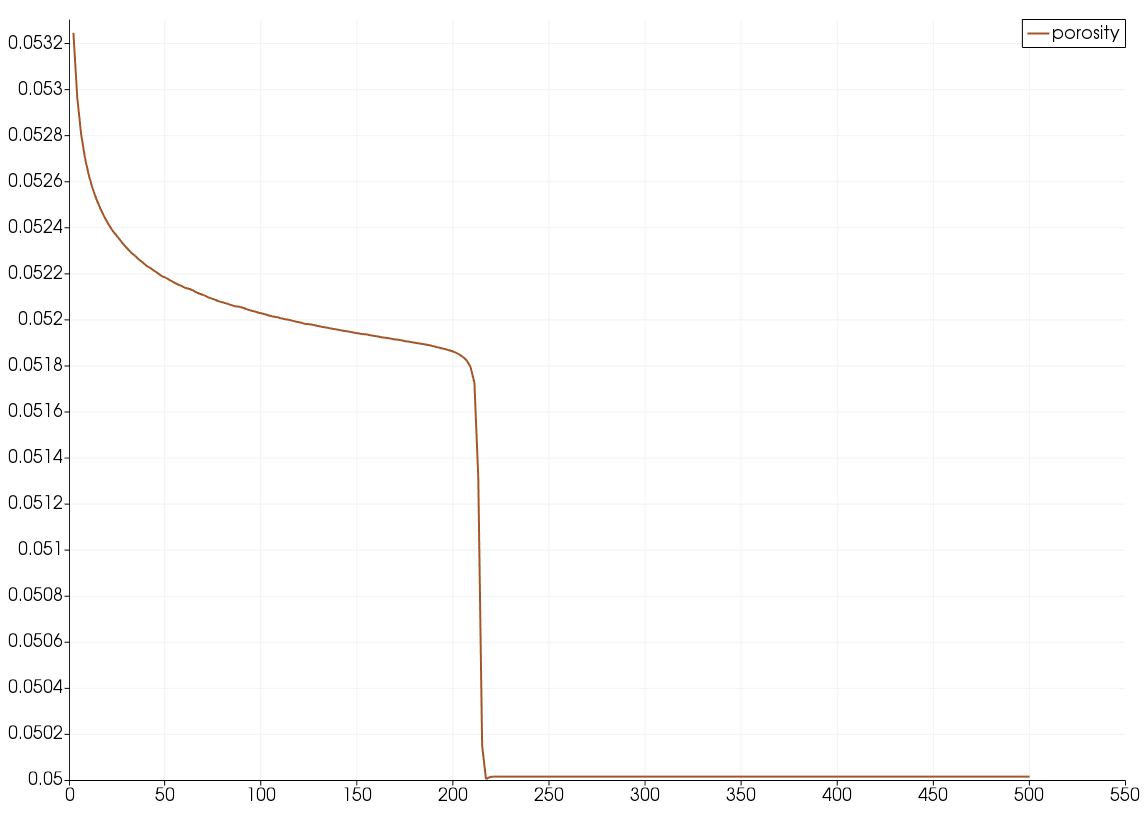
\includegraphics[width=.75\textwidth]{porosity}
\caption{Пористость в различных участках области} \label{fig:pic1}
\end{figure}

Значительная часть газа вступает в реакцию со скелетом. Это хорошо заметно на рисунке \ref{fig:pic2}, на котором приведена газонасыщенность в расчете с включенными реакциями (красный график) и без них (синий график).
При этом снижается и давление в области, что показано на рисунке \ref{fig:pic3}.

\begin{figure}[h!]
\centering
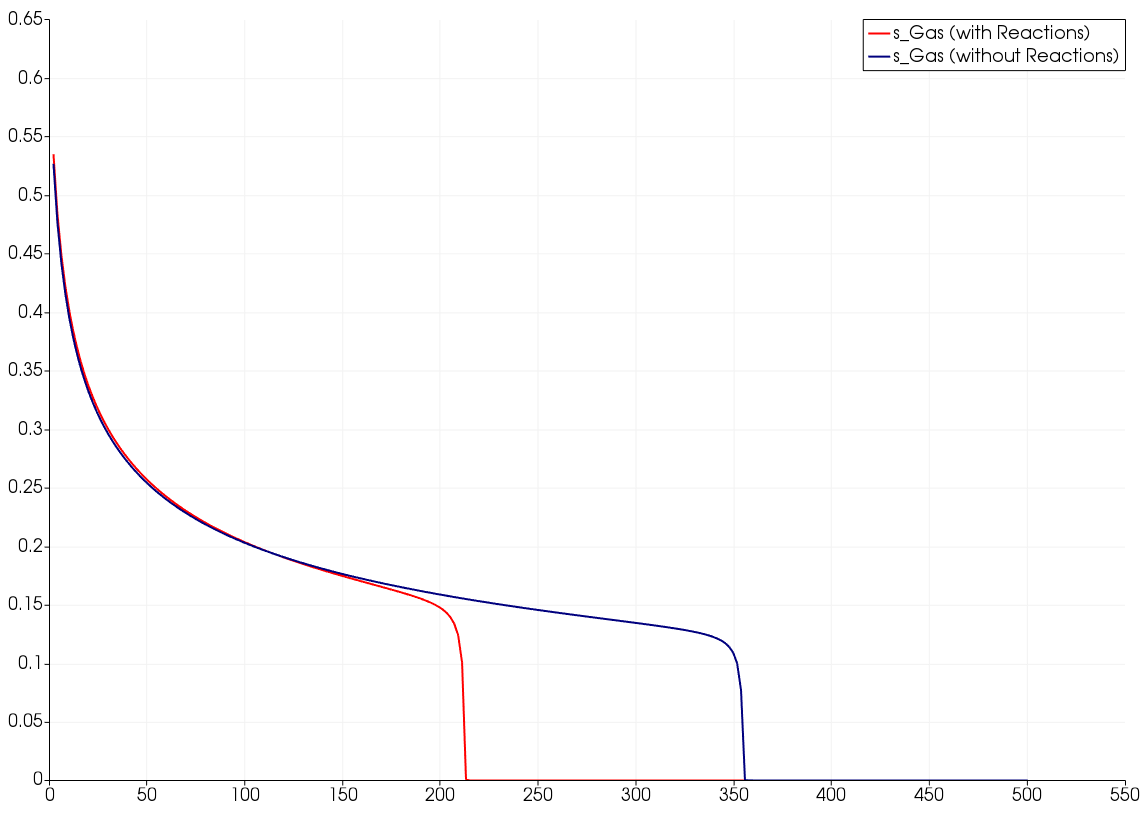
\includegraphics[width=.75\textwidth]{sG}
\caption{Газонасыщенность в области (с включенными реакциями и без)} \label{fig:pic2}
\end{figure}

\begin{figure}[h!]
\centering
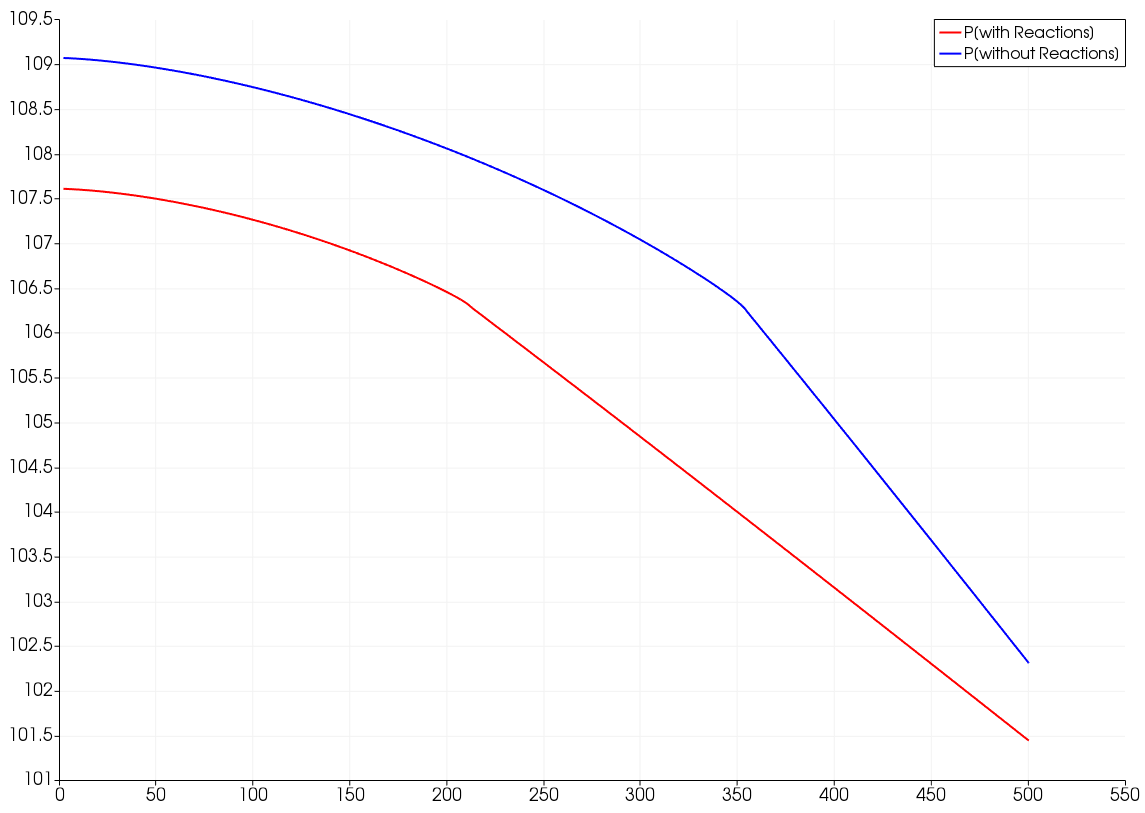
\includegraphics[width=.75\textwidth]{P}
\caption{Давление в области (с включенными реакциями и без)} \label{fig:pic3}
\end{figure}

\clearpage
\section{Выводы}

Предложенный метод Ньютона для расширенной системы уравнений равновесных химических реакций позволяет получать решения с произвольными начальными значениями глубин реакции, а также не требует корректировки длины шага. 

Модуль равновесных химических реакций был встроен в программный комплекс лаборатории флюидодинамики и сейсмоакустики МФТИ для моделирования многофазных многокомпонентных течений и протестировн на задаче закачки углекислого газа в водоносный пласт.

В будущем планируется объединить модуль расчета химического и фазового равновесия в единый блок.

\clearpage
\addcontentsline{toc}{section}{Список использованных источников}
%\section*{Список использованных источников}

\begin{thebibliography}{00} % библиография
\bibitem{shev}
\textit{Шевченко~А.\,В., Цыбулин~И.\,В., Скалько~Ю.\,И.}
Моделирование процессов фильтрации в коллекторах с переменной пористостью~//
Труды МФТИ,~---~2015.---~Т. 7, № 2(26). ~---~ С. 60--69.
\bibitem{vostrikov}
\textit{Ahusborde~E., Kern~M., Vostrikov~V.} Numerical simulation of two-phase multicomponent flow with reactive transport in porous media: application to geological sequestration of $\text{CO}_2$ ~//
ESAIM: Proceedings and surveys,~---~2015.---~V. 50.~---~Pp. 21--39.
\bibitem{kalit}
\textit{Калиткин~Н.\,Н., Альшина~Е.А.} Численные методы: в 2 кн. Кн. 1. Численный анализ. ~---
М.: Издательский центр <<Академия>>, 2013.~---~304~с.
\end{thebibliography}

\end{document}